
\subsection{Führungsschaufel}
\begin{tabular}{p{3.6cm}p{\textwidth-3.6cm-0.7cm}}
	\rule{0pt}{11pt}\textit{Typ}              & Führungsschaufel\\
	\rule{0pt}{11pt}\textit{Datum}:           & 13.03.2015   \\
	\rule{0pt}{11pt}\textit{Ort}:             & Werkstatt \\
	\rule{0pt}{11pt}\textit{Tester}:          & Pascal Roth und Matteo Trachsel  \\
	\rule{0pt}{11pt}\textit{Ziel des Testes}: & Das Ziel des Testes besteht darin, verschieden Führungsschaufeln zu testen und eine geeignete Befestigung zu finden. \\
	
	
	\rule{0pt}{11pt}\textit{Aufbau / Ablauf}: &
	Für den Test wurden aus einem 1 mm dicken Aluminiumblech, welches bereits auf die Breite des Förderbandes zugeschnitten wurde, verschieden Lange Stücke abgeschnitten. Da pro Tennisball zwei Führungsschaufeln vorne und hinten benötigt werden, gibt es zwei Möglichkeiten zur Gestaltung der Führungsschaufeln. Die erste Möglichkeit besteht darin, dass immer eine einzelne Schaufel für je vorne und hinten realisiert wird. Die zweite Möglichkeit besteht darin, dass man die hinter und die nächste vorne liegende Führungschaufel zusammen in einem Blechstück realisiert.\\
	
	
	\rule{0pt}{11pt}\textit{Fazit / Verbesserungs-\newline vorschlag}: &
	Durch den Versuch stellte sich heraus, dass es sich besser eignet, wenn zwei Führungsschaufeln zusammen in einem Blechstück realisiert werden. Wenn die Führungschaufelpaare mit dem UHU Kleber am vorderen Rand angeklebt werden, können sie immer noch den Radius der Wellen überfahren, ohne sich abzulösen. Zur Sicherheit können die Führungsschaufeln noch mit einem Klebeband befestigt werden. \\
\end{tabular}

\begin{figure}[h!]
	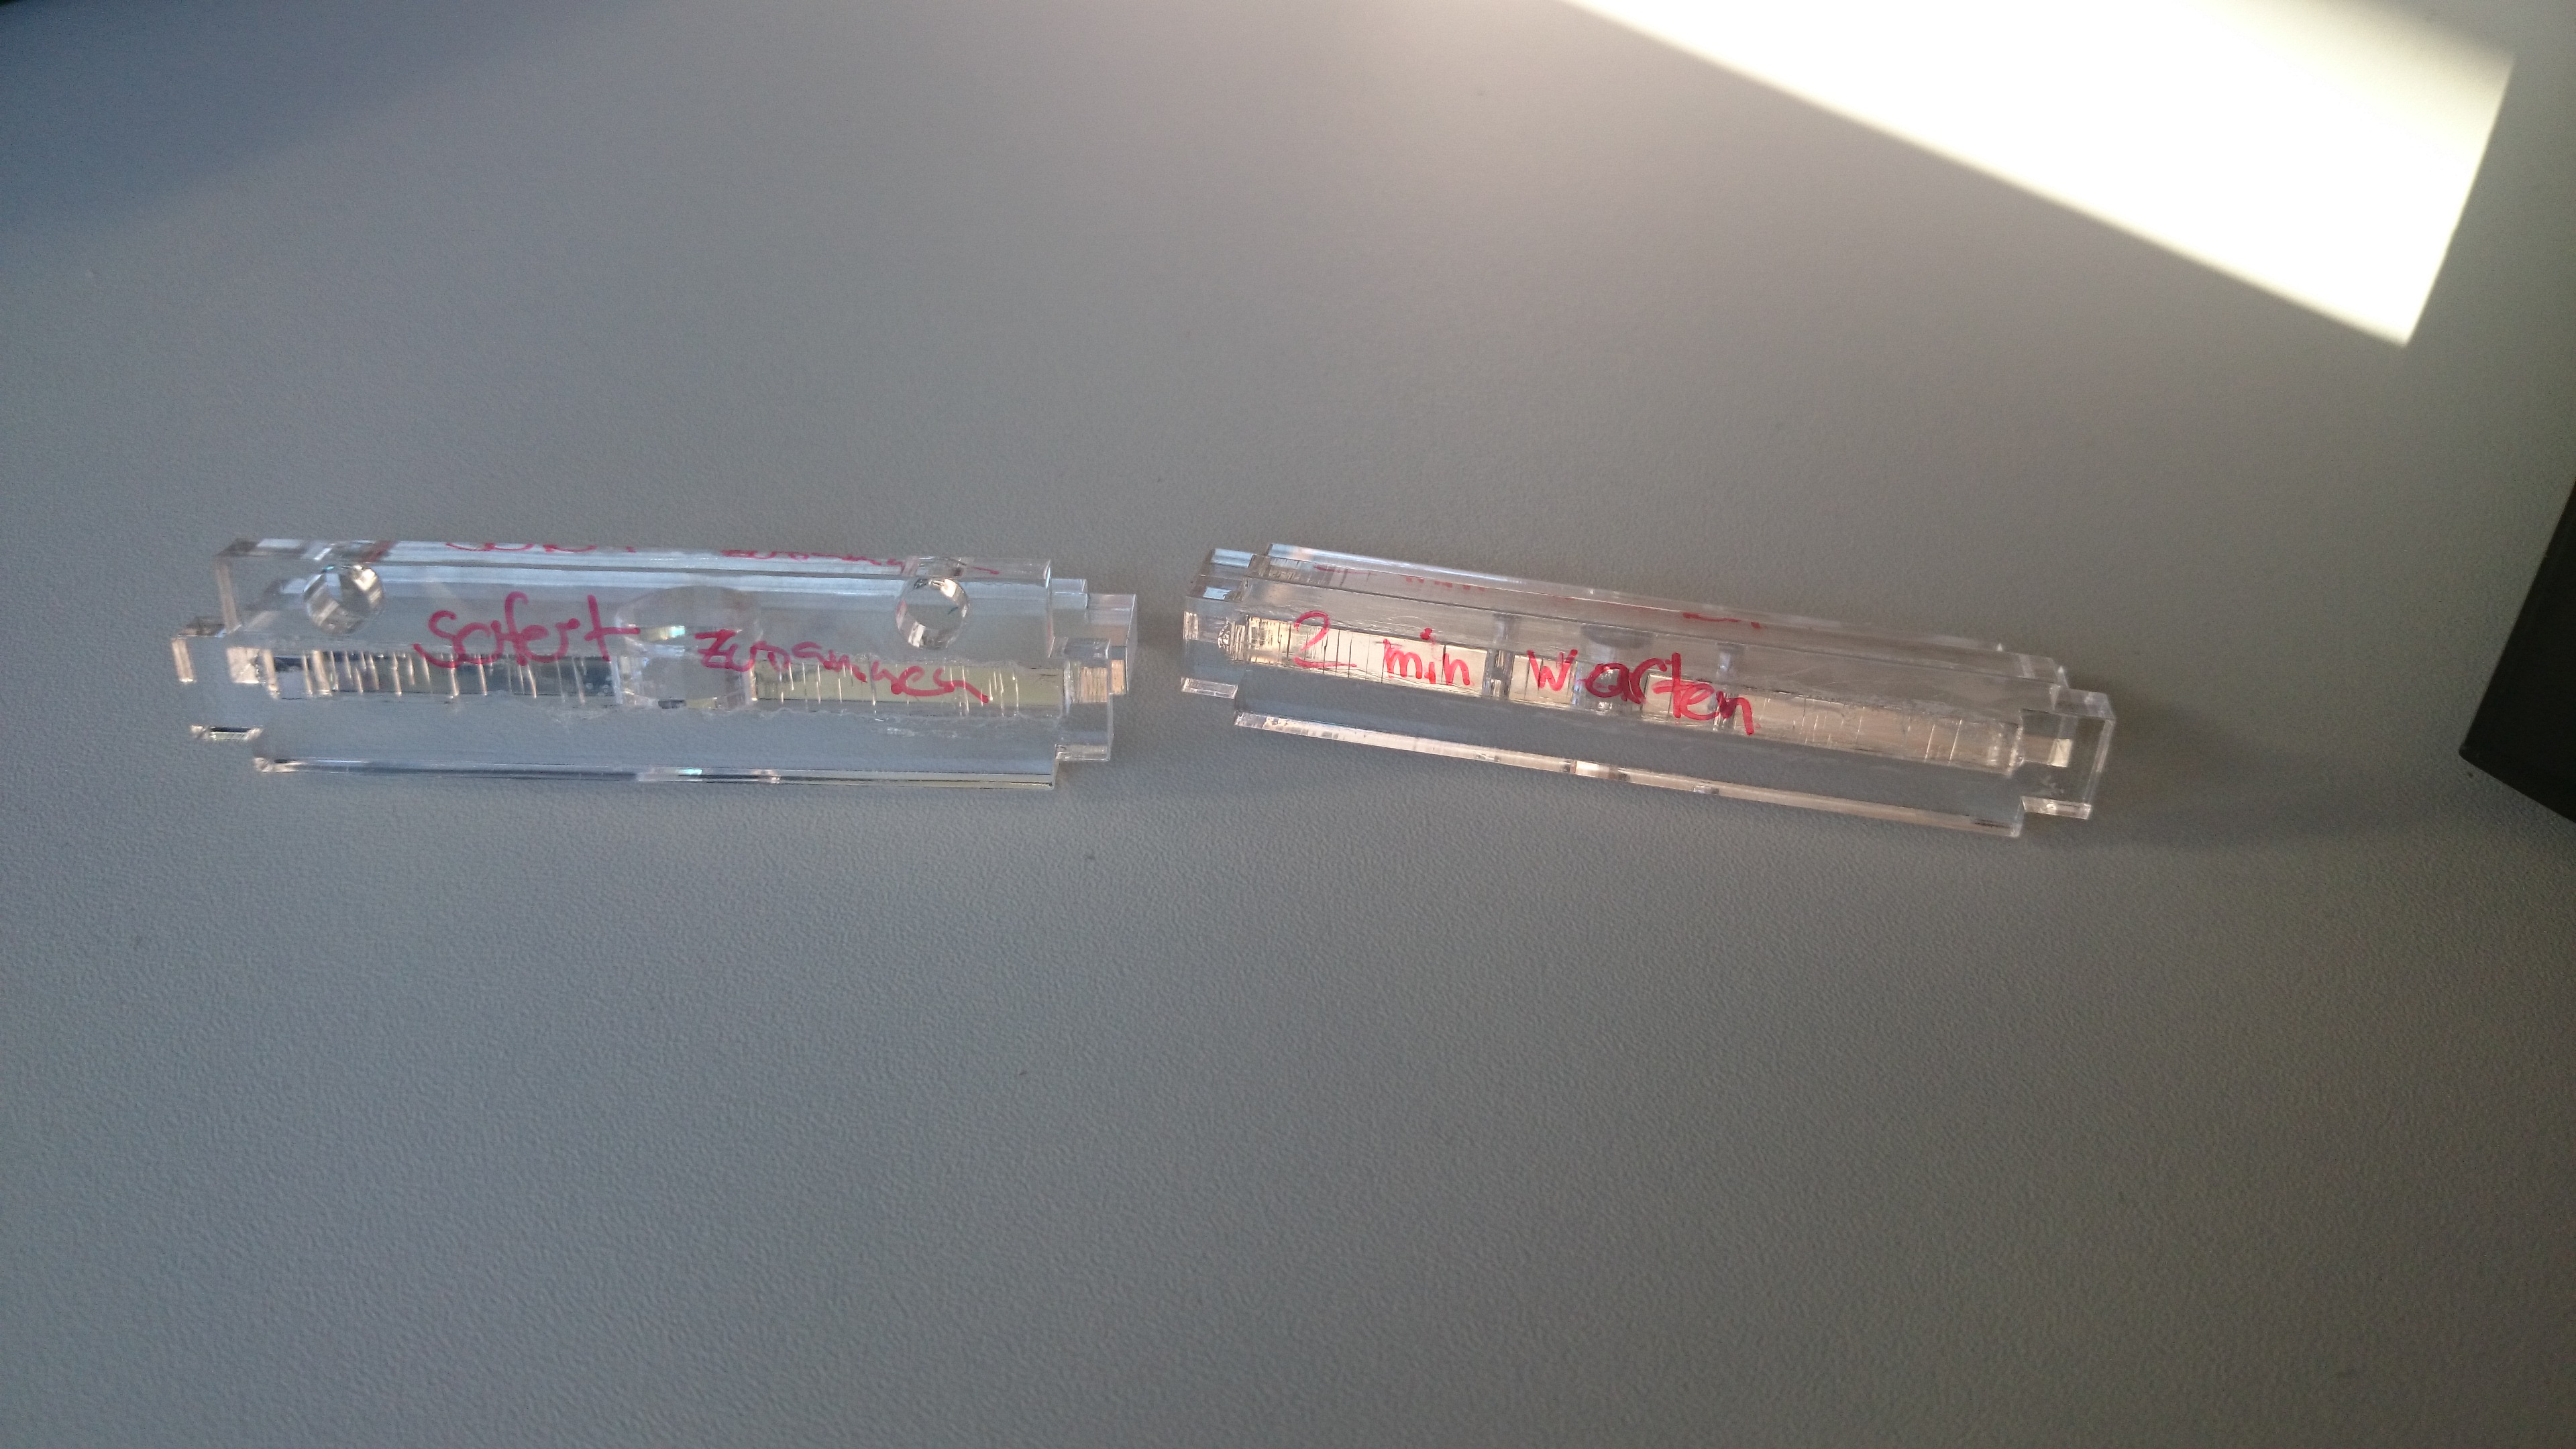
\includegraphics[width=0.9\textwidth,clip,trim=10cm 15cm 40cm 6cm]
	{Testberichte/Klebeversuch.jpg}
	\centering
	\caption{Förderband mit Führungschaufeln}
	\label{abb:Klebeversuch}
\end{figure}


